\begin{frame}{Recall}
    \begin{itemize}
        \item<1-> the input to a supervised learning algorithm is a training set ($x_{1:n}, y_{1:n}$), where
        \begin{itemize}
            \item<2-> $x_{1:n} = x_1,x_2,..., x_n$ shows input examples
            \item<3->  $y_{a:n}= y_1, y_2, ..., y_n$ shows corresponding labels
        \end{itemize}
        \item<4-> the goal of a learning algorithm is to return a function $f()$ that accurately maps input examples to their desired labels
        \uncover<5->{
        \begin{figure}
\centering
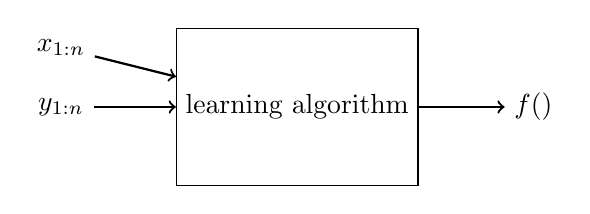
\begin{tikzpicture}

\node(x) at (0, 0) [] {$x_{1:n}$};
\node(y) at (0, -0.75) [] {$y_{1:n}$};


\node(lr) at (3,-0.75) [draw, minimum width=2cm, minimum height=2cm]{learning algorithm};

\draw[->,thick] (x) to (lr);
\draw[->,thick] (y) to (lr);

\node(f) at (6.0, -0.75) [] {$f()$};
\draw[->,thick] (lr) to (f);

\end{tikzpicture}
\end{figure}
        }
        \item<6-> how to measure if $f()$ works accurately?  
    \end{itemize}
\end{frame}
\begin{frame}{Loss Function}
\begin{itemize}
    \item<1->  \emph{Loss function $L(y,\hat{y})$}: It quantifies the loss suffered when predicting $\hat{\mathbf{y}}$ while the true label is $\mathbf{y}$
    
    \item<2-> given a labeled training set $(x_{1:n};y_{1:n})$, a per-instance loss function $L$ and a parameterized function $f(x;\Theta)$, we define the corpus-wide loss with respect to the parameters‚ as the average loss over all training examples:
    \begin{equation*}
        \mathcal{L}(\theta) = \frac{1}{n}\sum_{i=1}^{n}L(\hat{y},y_i),
    \end{equation*}
        \begin{equation*}
        \hat{y} = f(x_i;\Theta)
    \end{equation*}
\item<3-> in this view the training examples are fixed and the values of the parameters determine the loss
\end{itemize}
\end{frame}
\begin{frame}{Training as Optimization}
    \begin{itemize}
        \item<1-> the goal of the training algorithm is then to set the values of the parameters such that the value of $\mathcal{L}$ is minimized
        \begin{equation*}
            \hat{\Theta} = \text{argmin}_{\Theta} \mathcal{L}(\Theta) =\text{argmin}_{\Theta} \frac{1}{n}\sum_{i=1}^{n}L(\hat{y},y_i) 
        \end{equation*}
      \end{itemize}
\end{frame}
\begin{frame}{Common Loss Functions}
    \begin{itemize}
        \item Hinge (binary)
        \begin{itemize}
            \item<1-> for binary classification problems
            \item<2-> the classifier’s output is a single scalar $\hat{y}$ and the true output $y$ is in $\{-1,+1\}$
            \item<3-> the inference rule is prediction$= \text{sign}(\hat{y})$, and a classification is considered correct if $y \cdot \tilde{y} > 0$ 
            \item<4-> per-instance loss:
            \begin{equation*}
              L_{\text{hinge(binary)}} (\hat{y}, y) = \text{max}(0, 1 - y. \hat{y}) 
            \end{equation*}
        \end{itemize}
    \end{itemize}
\end{frame}
\begin{frame}{Common Loss Functions}
    \begin{itemize}
        \item Hinge (multi-class)
        \begin{itemize}
            \item<1-> let $\hat{y} =  \hat{y}_{[1]},\hat{y}_{[2]},..., \hat{y}_{[n]} $ be the model’s output vector, and $y$ be the one-hot vector for the correct output class
            \item<2-> the inference rule is defined as selecting the class with the highest score
             $\text{prediction}= \text{argmax}_{i}\hat{y}_{[i]}$
             \item<3-> if $t$ is the correct class and $k$ is the highest scoring class such that $k \neq t$ then loss is
                \begin{equation*}
              L_{\text{hinge(multiclass)}} (\hat{y}, y) = \text{max}(0, 1- (\hat{y}_{[t]}-\hat{y}_{[k]}))
            \end{equation*}
        \end{itemize}
    \end{itemize}
\end{frame}
\begin{frame}{Common Loss Functions}
    \begin{itemize}
        \item Log loss
        \begin{itemize}
            \item<1-> can be seen as a ``soft'' version of the hinge loss with an infinite margin 
             \item<2-> loss
                \begin{equation*}
              L_{\text{log}} (\hat{y}, y) = \text{log}(1+\text{exp}(-(\hat{y}_{[t]}-\hat{y}_{[k]}))
            \end{equation*}
        \end{itemize}
    \end{itemize}
\end{frame}
\begin{frame}{Common Loss Functions}
    \begin{itemize}
        \item<1-> binary cross entropy (logistic loss)
        \begin{itemize}
            \item<2-> used for binary classification with conditional probability outputs. 
            \item<3-> assumes a set of two target classes labeled 0 and 1, with a correct label $y\in \{0, 1\}$
            \item<4-> the model’s output $\tilde{y}$ is transformed using the sigmoid function
            \begin{equation*}
                \sigma(x) = \frac{1}{1+e^{-x}}
            \end{equation*}
            \item<5-> then $\hat{y} = \sigma(\tilde{y}) = P(y=1|x)$
            \item<6-> inference rule: prediction$=0$ if $\hat{y}<0.5$ and prediction$=1$ if $\hat{y}>=0.5$
             \item<7-> loss
                \begin{equation*}
              L_{\text{logistic}} (\hat{y}, y) = -y\text{log}(\hat{y}) -(1-y)log(1-\hat{y})
            \end{equation*}
            \item<8->  is useful for estimating class conditional probability for a binary classification problem
            \item<9-> we assume that the output layer is transformed using sigmoid
        \end{itemize}
    \end{itemize}
\end{frame}
\begin{frame}{Training as Optimization}
    \begin{itemize}
        \item<1-> the goal of the training algorithm is then to set the values of the parameters such that the value of $\mathcal{L}$ is minimized
        \begin{equation*}
            \hat{\Theta} = \text{argmin}_{\Theta} \mathcal{L}(\Theta) =\text{argmin}_{\Theta} \frac{1}{n}\sum_{i=1}^{n}L(\hat{y},y_i) 
        \end{equation*}
      \item<2-> the above optimization attempts to minimize the loss at all costs, which may result in overfitting the training data 
      \end{itemize}
\end{frame}
\begin{frame}{Regularization}
    \begin{itemize}
     
        \item<1-> to counter that we define a regularization term $R(\Theta)$ taking as input the parameters and returning a scalar that reflect their ``complexity,'' which we want to keep low
        
        \item<2-> training 
        \begin{equation*}
            \hat{\Theta} = \text{argmin}_{\Theta} \mathcal{L}(\Theta) =\text{argmin}_{\Theta} \frac{1}{n}\sum_{i=1}^{n}L(\hat{y},y_i) 
        \end{equation*}
     
     \item<3-> training with regularization
        \begin{equation*}
            \hat{\Theta} = \text{argmin}_{\Theta} \mathcal{L}(\Theta) =\text{argmin}_{\Theta} \left( \frac{1}{n}\sum_{i=1}^{n}L(\hat{y},y_i)  + \lambda R(\Theta) \right)
        \end{equation*}
    \end{itemize}
\end{frame}
\begin{frame}{Regularization}
    \begin{itemize}
        \item<1-> intuitively we would like to drive the learner toward natural solutions, in which it is OK to mis-classify a few examples if they don’t fit well with the rest
        \begin{equation*}
            \hat{\Theta} =\text{argmin}_{\Theta} \left( \frac{1}{n}\sum_{i=1}^{n}L(\hat{y},y_i)  + \lambda R(\Theta) \right)
        \end{equation*}
        \item<2-> regularization term considers the parameter values, and scores their complexity
        \item<3-> in practice the regularizers equate complexity with large weights and work to keep the parameter values low 
        
    \end{itemize}
\end{frame}
\begin{frame}{Common Regularization Functions}
    \begin{itemize}
        \item<1-> $L_2$ regularization (a.k.a. gaussian prior or weight decay): It keeps the sum of the squares of the parameter values low
        \begin{equation*}
            R_{L_2}(W) = ||W||_2^2 = \sum_{i,j}{(W_{[i,j]})^2}
        \end{equation*}
        \item<2-> the learner will prefer to decrease the value of one parameter with high weight by $1$ than to decrease the value of ten parameters that already have relatively low weights by $0.1$ each
    \end{itemize}
\end{frame}
\begin{frame}{Common Regularization Functions}
    \begin{itemize}
        \item<1-> $L_1$ regularization (a.k.a. sparse prior or lasso): It keeps  the sum of the absolute values of the parameters low
        \begin{equation*}
            R_{L_1}(W) = ||W||_1 = \sum_{i,j}{|W_{[i,j]}|}
        \end{equation*}
        \item<2-> the learner will prefer to decrease all the non-zero parameter values toward zero
    \end{itemize}
\end{frame}
\begin{frame}{Common Regularization Functions}
    \begin{itemize}
        \item<1-> Elastic-Net: combines both $L_1$ and $L_2$ regularization
        \begin{equation*}
            R_{\text{elastic-net}}(W) = \gamma_1 R_{L_1}(W) + \gamma_2 R_{L_2}(W)
        \end{equation*}
        \item<2-> dropout: will be discussed later
    \end{itemize}
\end{frame}